\chapter{Datenquelle 2: EASA und Easy Access Rules}

    \section{European Union Aviation Safety Agency}

% \begin{quote}
% \textcolor{red}{Einführung zur EASA. Neue Position und Bedeutung für den Prozess. Was sind Easy Access Rules und welche Bedeutung haben sie für uns. Hard law / Soft law. Added benefit durch AMC/GM}
% \end{quote}
% \begin{quote}
% \textcolor{green}{1-2 Seiten}
% \end{quote}

Nach dem informellen Zusammenschluss paneuropäischer nationaler Luftfahrtbehörden (\acs{NAA}), zwecks der Standardisierung von Flugzeugzertifizierungsprozessen ab 1970\footnote{\acf{JAA}} erkannten \ac{EU} Initiativen 1996 bereits den Bedarf einer zentralen europäischen Luftfahrtbehörde.
Im Jahre 1990 definierte die Kommission Ziele an eine ,,Harmonisierung der technischen Vorschriften und Verfahren für Zivilluftfahrzeug[!]``\cite{kom_90_442}, welche unter anderem anregten: 

\begin{quote}
    ,,Dieser Ansatz sollte langfristig zur Schaffung einer einheitlichen Europäischen Luftfahrtbehörde führen, wodurch eine völlige Harmonisierung der Sicherheitsnormen und deren konsequente Durchführung sichergestellt wären.``\footnote{Im Rahmen dieses Vorschlags war die Schaffung einer solchen Behörde explizit von dem Rahmen des Dokuments ausgenommen (siehe gleicher Absatz)} \cite[Begr. Art. 7 Abs. 2]{kom_90_442}
\end{quote}
Auf Basis dieser Bemühungen wurde die \acf{EASA}\footnote{Zunächst definiert als European Aviation Safety Authority \cite[2]{easa_framework}} im Jahre 2002 durch die Verordnung \vo{VO}{EG}{1592/2002} offiziell als Einrichtung der \ac{EU} gegründet und würde ein Jahr später ihre zuvor definierte Arbeit aufnehmen.
Nach dieser Definition sollte die \ac{EASA} zunächst die Zusammenarbeit der europäischen \acsp{NAA} koordinieren und dessen Meinungen im Umfeld der \ac{EU}-Organe repräsentieren. 
\cite[§4.3]{easa_coman2018}



\subsubsection{Aufgaben der EASA}

Im Rahmen der Verordnungen \vo{VO}{EG}{216/2008}\textdagger{} -- und später \vo{VO}{EU}{2018/1139} -- wurden die Aufgaben, der innere Aufbau, die Arbeitsweise und die Finanzvorschriften der Agentur dargelegt.
Die Hauptaufgaben der \ac{EASA} belaufen sich auf der Erstellung von Gutachten zur zivilen Flugsicherung in Europa; der Unterstützung der Kommission durch die Ausarbeitung von Maßnahmen\footnote{welche zur Durchführung der in der Verordnung definierten Ziele helfen} und Hilfestellungen bei technischen Fragen\footnote{bspw. im Zusammenhang mit Bau- und Konstruktionsvorschriften}; der Ausführung von benötigten Inspektion und Untersuchungen\footnote{im Sinne der definierten Ziele dieser Verordnung}; und -- unter der Erweiterung in 2018\footnote{nach \vo{VO}{EU}{2018/1139}} -- sicherheitsrelevante Aspekte der Gefahrenabwehr, wie Cybersicherheit; und Umweltschutz. \cite{2008R0216_summary, 2018R1139_summary}

Die Anforderungen sowie dessen Durchsetzungsprozesse in Bezug auf \atmans-Ausrüstung werden in den Artikeln 40--47 der \vo{VO}{EU}{2018/1139} definiert und durch weitere Publikationen der \ac{EASA} unterstützt.
        
        \pagebreak

        \subsection{Annehmbare Nachweisverfahren}

        Die \ac{EASA} ist nach der Anforderung \textsf{ATM/ANS.AR.A.015(a)}\footnote{aus dem Anhang II der \vo{DVO}{EU}{2017/373}} angehalten, annehmbare Nachweisverfahren (engl. Accepted Means of Compliance (\acs{AMC})) zu entwickeln, welche zur Bewertung der Compliance herangezogen werden können und dessen Abdeckung eine vollständige Abdeckung der zugrundeliegenden einschlägigen Verordnung garantiert. 
        \cite[Anh. II]{2017R0373}

    \subsubsection{Alternative Nachweisverfahren}

        Sollten die \textit{Annehmbaren Nachweisverfahren} der \ac{EASA} nicht zur Erfüllung der Compliance infrage kommen, so können Diensteanbieter auch auf selbstdefinierte \acf{AltMOC} zurückgreifen.
        Es fällt folglich in den Aufgabenbereich der zuständigen Behörde, ein System zur durchgängigen Bewertung  vorgelegter \acp{AltMOC} zu entwickeln und feststellen zu können, ob diese alle Anforderungen einschlägigen Verordnungen erfüllen.
        \cite[Anh. II \textsf{ATM/ANS.AR.A.015(b-e)}]{2017R0373}
        
        \subsection{Guidance Material}

    Ähnlich wie bei der Erarbeitung von \textit{Annehmbaren Nachweisverfahren} entwickelt die \ac{EASA} sogenanntes \acf{GM}\footnote{Im Folgenden auch ,,Anleitungen``}.
    Diese Dokumente sollen zusammen mit den \acp{AMC} helfen, klaren Rahmenbedingungen für die Umsetzung der Anforderungen sowie deren Kontrolle zu definieren
    \cite[7]{easa_2017001r}.
    Diese Anleitungen können u.a. Beispiele der Umsetzungen von Standards, Begriffsdefinitionen oder weitere Informationen sein, welche bei der Umsetzung der entsprechenden Durchführungsbestimmungen dazugezogen werden können.

        \subsection{Rechtsetzungsprozess}

    Um die erarbeiteten Durchführungsbestimmungen und Zusatzmaterialien\footnote{\ac{AMC} und \ac{GM}} in den gesetzlichen Rahmen publizieren zu können, bedarf es der \ac{EASA} einem strukturierten Rechtsetzungsprozess\footnote{gefordert durch Art. 52(1) \vo{VO}{EG}{216/2008}}.
    Unter diesem arbeitet die \ac{EASA} Themen ihrer definierten Rechtsetzungsagenda\footnote{\href{https://www.easa.europa.eu/en/document-library/rulemaking-programmes}{https://www.easa.europa.eu/en/document-library/rulemaking-programmes}}$^,$\footnote{\href{https://www.easa.europa.eu/en/domains/safety-management/european-plan-aviation-safety}{https://www.easa.europa.eu/en/domains/safety-management/european-plan-aviation-safety} (nach 2018)} in Gesetzesvorschläge aus und publiziert unterdessen Entwürfe und \acfp{NPA}, um den Prozess eng mit Stakeholder:innen zu koordinieren.
    Auf Basis des Feedbacks wird anschließend die finale Fassung des Textes entworfen und der Kommission zur Adoption überlassen. \cite[3]{easa_2017001r} 
        
\pagebreak
\noindent
Die Einrichtung der Agentur nach diesem Plan ist im Vergleich mit anderen \ac{EU} Agenturen sehr ambitioniert und spiegelt wider, wie Agenturen einen immer wichtigeren Stellenwert in den legislativen Prozessen der \ac{EU} einnehmen. 
Durch die \ac{EASA}-Grundverordnung erhält die Agentur die rechtliche Grundlage, Durchführungsbestimmungen und Guidelines zu definieren, welche in ihrer rechtlichen Wirksamkeit nicht von anderen Rechtsakten zu unterscheiden sind.
Weiter benötigen \ac{EU}-Mitgliedsstaaten, welche sich gegen die Durchsetzung von Anforderungen der \ac{EASA} entscheiden, dessen explizite Zustimmung.   
\cite[260]{easa_administrative_innovation}
        

        \subsection{Easy Access Rules}

\acf{EAR} sind eine Publikation der \ac{EASA}, welche die drei oben definierten Parts von Durchführungsbestimmungen, \acp{AMC} und \acp{GM} kombiniert und zu einem Thema gesammelt veröffentlicht.
Hiermit soll Nutzer:innen ein einfacher, übersichtlicher Überblick über alle verfügbaren Ressourcen sowie deren Verbindungen untereinander ermöglicht werden.

\medskip
\noindent
    Die einzelnen Werke werden dabei im mehreren Formate veröffentlicht:
    \begin{itemize}
        \item Einem PDF Format als Printmedium;
        \item einer interaktiven Weboberfläche, welche die Inhalte entsprechend abbildet und das Suchen nach Stichwörtern oder anderen Kriterien ermöglicht;
        \item  und den zugrundeliegenden Daten in Form einer maschinenlesbaren XML-Datei. \cite{easa_xml_export}
    \end{itemize}



\subsubsection{Definition nach FRBR}

    Im Rahmen der behandelten Definitionen aus der Studie zu funktionalen Anforderungen bibliografischer Datensätze \acs{FRBR} (siehe \ref{frbr}) bilden die \textit{Easy Access Rules} eine weitere \textit{Manifestation} des bestehenden \textit{Werkes} über die Durchführungsbestimmungen.
    Auch wenn die \ac{EAR} den Umfang bestehender \textit{Manifestationen} inhaltlich um \textit{Annehmbare Nachweisverfahren} und \textit{Guidance Material} erweitern, so ändern sie nicht dessen intellektuelle Schöpfung.
    Der Sinn, die ursprünglichen Werke und deren verbundene Zusatzinhalte zugänglicher zu machen, geht hierbei mit der Integrität\footnote{auch wenn nicht verbindlich definiert} der intellektuellen Schöpfung einher und stellt keine Interpretation dieses Werkes dar.

        \pagebreak
    \section{EASA eRules Plattform}

    Die \ac{EASA} eRules Plattform ist ,,einheitliche, einfach zugängliche, online Datenbank für alle in der Luftfahrt anwendbaren Regeln für Stakeholder im europäischen Luftraum``.
    \cite[5]{easa_xml_doc}

    Als ein Produkt dieser Plattform werden die sogenannten Easy Access Rules definiert und bis dato (24.6.22) in zwei Formaten veröffentlicht. 

    
Am 26. Januar 2023 veröffentlichte die EASA die Entscheidung, Easy Access Rules fortan auch in einem maschinenlesbaren XML Format Endnutzern bereitzustellen. \cite{easa_xml_publication}


\subsection{Informationsarchitektur}
\label{ch:easa_arch}

    Im Rahmen der eRules Plattform und des maschinenlesbaren \ac{XML} Formates, werden Inhalte in kleine sogenannte ,,Topics`` unterteilt.
    Ein Topic repräsentiert eine \ac{EU} Durchführungsbestimmung (siehe \ref{ch:ir}); eine \ac{EU} Delegierte Bestimmung; ein Annehmbares Nachweisverfahren der \ac{EASA}; \ac{EASA} Guidance Material; oder sog. \ac{EASA} \acf{CertS}\footnote{(CS) wegen Überschneidung mit \acf{CS} geändert}. \cite[S. 5f]{easa_xml_doc}
    
Topics werden repräsentativ ihrer konzeptuellen Beziehungen zwischen den unterschiedlichen Topics in der baumartigen Struktur abgebildet.
Hierbei werden Topics, welche Verordnungen oder \ac{CertS} abbilden meist auf einem strukturell höheren Level und alle diesem zugeordneten Topics wie. \acsp{AMC}, \acsp{GM}, oder anderen Gesetzesgrundlagen dargestellt.

        
        \subsubsection{Publikationsformat}

    Die für die Publikation der maschinenlesbaren Dokumente wählte die \ac{EASA} die von \acf{MS} etablierte und standardisierte \acf{OPC}\footnote{\acs{ECMA}-376, ISO/IEC 29500-2}.
    Dieser Standard ist Teil der Familie an \ac{XML} Schemata, welche gemeinsam als \acf{OOXML} bezeichnet werden\footnote{ ISO/IEC 29500} und \ac{XML} Semantiken für Textverarbeitungs-, Tabellen\-kal\-ku\-lations- und Präsentationsdokumente -- oder hiermit konformen Dokumenten -- bereitstellen. 
    \cite[vii]{easa_opc_iso} 
    Die Besonderheit dieses Formates ist es, dass das Gesamtdokument in kleineren Parts\footnote{gemäß 6.2 ISO/IEC 29500-2 \cite{easa_opc_iso}} strukturiert wird, welche nach der Definition der \ac{OPC} -- ähnlich wie ein Archiv -- in ein Gesamtdokument zusammengefasst werden.
    Hierauf basierende Standards, wie \ac{OOXML}, definieren meist nur die Struktur einzelner Parts, was eine konforme Erweiterung des Gesamtdokumentes durch weitere Parts problemlos ermöglicht.   
    Dies bedeutet unter anderem, dass valide Dokumente Teil von größeren Gesamtdokumentes sein können, wessen weitere Parts keinen Einfluss auf dessen Benutzung als konformes Open Office-Dokument nehmen.
    Genau von dieser Eigenschaft hat die \ac{EASA} Gebrauch gemacht und ihre Informationen auf zwei Arten in das Gesamtdokument integriert:

    \pagebreak
            \subsubsection{Anforderungsinhalte}

    Inhalte von Topics werden unter Release 1.0.0 der eRules \ac{XML} Spezifikation als ,,opaque data structure`` angesehen.
    Dies bedeutet, dass im Zug dieses Releases keine inhaltliche Struktur der Inhalte der Topics definiert wurde.
    Es bleibt jedoch den Anwender:innen überlassen, Implementationen auf die Angaben innerhalb des beschriebenen \acs{OOXML} Formates zu stützen.
    \cite[6]{easa_xml_doc}

    % \medskip
    Nach diesem Standard sind die textuellen Inhalte der einzelnen Topics Teil des Textverarbeitungsdokumentes\footnote{Part Name: "\textit{/word/document.xml}"} und lassen sich damit auch über eine grafische Textbearbeitungsoberfläche (bspw. \ac{MS} Word) einsehen und bearbeiten.
    Hierbei werden Textinhalte des Dokumentes so strukturiert, dass die einzelnen Entitäten voneinander isoliert und über eine -- innerhalb des Dokumentes -- lokal einzigartige ID, eindeutig identifizierbar gemacht werden.
    So können die Inhalte bei Bedarf beliebig bearbeitet werden, ohne die Struktur der Topics oder die Integrität anderer strukturellen Verweise zu gefährden.
            % Außerdem ist es so möglich, Einträge in den Metadaten auf die entsprechenden Anforderungsinhalte verweisen zu lassen. 

            \subsubsection{Metadaten}

    % Zusätzlich zu den Inhalten ermöglicht es der \ac{OOXML} Standard, weitere Parts an das Textdokument anzuhängen.
    Die \ac{EASA} nutzt zusätzlich die Möglichkeit, konforme \ac{OOXML} um eigene Parts zu erweitern, um das inhaltliche Dokument mit Metadaten der einzelnen Topics, auf Basis des internen \ac{EASA} \ac{CCMS}, zu bereichern.
    Diese Metadaten enthalten interne Informationen zu der Struktur des Dokumentes und den einzelnen Anforderungen und stehen dem Endnutzer in Form eines \ac{OPC} Parts  zur Verfügung.
    Dessen Struktur beruht auf einem eigenen \ac{XML} Schema, welches in der entsprechenden Dokumentation der \ac{EASA} definiert ist.

\pagebreak
\subsection{Analyse der Metadaten}
\label{ch:easa_anal}

    Die für diese Analyse relevanten Attribute, welche Metadaten der oben definierten Topics beschreiben, werden im Rahmen der Dokumentation unter der Gruppe ,,\textsf{topic-metadata}``\footnote{\ac{XSL} Attribute Group} festgehalten.
    Diese Gruppe beinhaltet die im Folgenden analysierte Attribute.\footnote{Alle beschriebenen Attribute werden durch den Typ String ohne jegliche Einschränkungen abgebildet und im Folgenden durch ,,[AttributName] Attribut`` oder -- gemäß dem XPath Standard -- ,,@[AttributName]`` referenziert} \cite[9]{easa_xml_schema}

    \subsubsection{ERulesId}

Die \textit{ERulesId} stellt eine -- über alle publizierten Dokumente hinweg -- einzigartige Kennung eines jeden Topics dar.
Dies ermöglicht eine einfache, einheitliche Referenzierung von Topics unabhängig von deren zugehörigem Dokument.
Die \ac{EASA} garantiert diesbezüglich, dass die Id über den gesamten Lifecycle des Topics unveränderlich sind. \cite[17]{easa_xml_doc}

In Bezug auf die Impactanalyse, bietet dieses Attribut einen großen Vorteil, da die definierten Anforderungen an eine \textit{Eindeutige Kennung} (vgl. \ref{model_anforderungen}) bereits für alle Topics der \ac{EASA}\footnote{Darunter, durch \ac{IR}, auch \atmans Anforderungen} erfüllt sind.
% \medskip
\begin{quote}
Beispiel:
\textsf{ERulesId="{}ERULES-1891294191-107"}
\end{quote}

% A unique identifier attribute for every topic in the exported XML file, which allows the unique identification of a topic across all the exported XML files from EASA. The ERulesId value is unchanged: • from publication to publication, everywhere the topic is reused; and • from version to version, throughout the entire life cycle of the topic.  
    
    \subsubsection{Domain / Activity Type}

Die \textit{Domain} und der \textit{Activity Type} eines Topics bezeichnen dessen Aufgabenbereich sowie die technische Beschreibung der darin vollbrachten Aufgabe \cite[S. 18]{easa_xml_doc}.
Im Umfang der nach \vo{VO}{EU}{2018/1139} i.V.m. \vo{VO}{EU}{628/2013} definierten Aufgabenbereiche kann in unserem Falle immer die \textit{Domain} \atmans angenommen werden.

Mögliche Werte des \textit{ActivityType}-Attributs beinhalten u.a.\footnote{Nicht holistische Liste an Beispielen \cite[vgl.][S.18 -- 19]{easa_xml_doc}} die unter \atmans definierten Aufgaben (siehe \ref{beg:atmans}).
Sie geben in der folgenden Analyse Auskunft darüber, für welche \atmans Ausrüstungen die Topics eine Relevanz aufweisen.
Dies kann u.a. genutzt werden, um die Relevanz neuer Anforderungen zu ermitteln oder irrelevante Anforderungen im Nachweisführungsprozess anderer Ausrüstungen auszuschließen.  

\begin{quote}
    Beispiel:
    \textsf{ActivityType="Meteorological Services (MET)"}
\end{quote}
   
    \subsubsection{AircraftCategory / AircraftUse / RegistryState}

Die Attribute \textit{AircraftCategory}, \textit{AircraftUse} und \textit{RegistryState} beziehen sich auf die Klassifizierung und Zuordnung von Anforderungen an Flugzeuge und haben für \atmans Equipment kein Gewicht\footnote{Eine vorangehende Analyse hat ergeben, dass diese Attribute in den \atmans Dokumenten nicht verwendet werden}. \cite[20, 21, 26]{easa_xml_doc}
    
    \subsubsection{AmendedBy}

Im Falle von Änderungen des \textit{Topics} referenziert dieses Attribut die lokale Konsolidierung der \ac{EAR}
\cite[21]{easa_xml_doc}.
Nach deren Publikation unbearbeitete \textit{Topics} führen den Wert \textsf{"{}Initial issue;"}

\begin{quote}
    Beispiel:
    \textsf{AmendedBy="{}Amendment 1;"}\footnote{Die Kennung der Änderung bezieht sich ausschließlich auf die aktuelle \ac{EAR}}
\end{quote}
    
    \subsubsection{ApplicabilityDate / EntryIntoForceDate }

Die Attribute \textit{Applicability-} und \textit{EntryIntoForceDate} beschreiben im Falle von Topics, welche sich auf Durchführungsbestimmungen beziehen, den entsprechenden zeitlichen Rahmen von deren Gültigkeit.
Das \textit{ApplicabilityDate} repräsentiert dabei -- unabhängig von dem juristischen Wortlaut -- den letzten Tag der Übergangsperiode. 
Das \textit{EntryIntoForceDate} hingegen repräsentiert das offizielle Inkrafttreten rechtlicher Durchführungsbestimmungen, nach welcher die rechtliche Bindung der in dem Topic abgebildeten Anforderung beginnt.
\cite[21]{easa_xml_doc}
Mangels rechtliche Bindung verfügen Topics in Bezug auf \acsp{AMC} oder \ac{GM} nicht über diese Attribute.\footnote{Strukturell sind alle Topics gleich, der Wert bleibt lediglich leer}
    
    \subsubsection{EquivalentForeignRegulation}

Das Attribut \textit{EquivalentForeignRegulation} äquivalente Regularien von nicht \ac{EU} Mitgliedstaaten.
Diese Informationen werden -- nach Angaben der \ac{EASA} -- hauptsächlich zum Angleichen von Designstandards von Flugzeugdesigns genutzt \cite[22]{easa_xml_doc}, finden nach eigener Auswertung aber auch im \atmans Sektor Anwendung, um bspw. international gemeinschaftliche Nachweisverfahren zur Luftdatenverarbeitung zu etablieren (siehe Beispiel).

\begin{quote}
    Beispiel:
    \textsf{EquivalentForeignRegulation="{}AC No: 20-153B;"}\footnote{Referenziert \ac{FAA}: \ac{AC} 20-153B - ,,Acceptance of Aeronautical Data Processes and Associated Databases``}$^,$\footnote{Semikolon beschreibt mögliche Auflistung mehrerer (durch Semikola getrennte) Einträge }
\end{quote}

    \subsubsection{ICAOReference}

Verweist auf -- im Rahmen des \textit{Topics} -- relevante \ac{ICAO} \acp{SARP}. 
\cite[23]{easa_xml_doc}

\begin{quote}
    Beispiel:
    \textsf{ICAOReference="{}Annex 11; Annex 19;"}
\end{quote}
    
    \subsubsection{Keywords}

    Die Verwendung des \textit{Keyword} Attributs ist nach der offiziellen Dokumentation nicht genau festgelegt.
    Es wird verwendet, um weitere Metadaten anzuhängen oder eine Kategorisierung anhand einzelner Schlüsselwörter umzusetzen.
\cite[23--26]{easa_xml_doc}
    \begin{quote}
    Beispiel:
    \textsf{Keywords="{}Safety measures; safety tracking"}
\end{quote}

    \subsubsection{RegulatedEntity}

Die regulierte juristische Person (\textit{regulated entity}) definiert, an wen die -- im \textit{Topic} definierte -- Anforderung gerichtet ist und wer diese im gleichen Zug zu erfüllen hat.
Diese \textit{Entities} beschreiben entweder Stakeholder:innen der Luftfahrtindustrie oder der zuständigen Behörde\footnote{hier \ac{EASA}} \cite[26]{easa_xml_doc}.

Im Rahmen der \atmans Anforderungen kann dieses Attribut auch die Anbieter der definierten \atmans Dienste definieren.
Diese Informationen können so eine sehr gute Abbildung erzeugen, welche Bereiche im \atmans Sektor von entsprechende \textit{Topics} reguliert werden.  
    \begin{quote}
    Beispiel:
    \textsf{RegulatedEntity="{}ATS provider; ANS provider;"}
\end{quote}

    
    \subsubsection{Regulatory Source}

Die Funktion dieses Attribut beschreibt -- analog zur Definition aus \ref{model_anforderungen} -- die Regulatorische Quelle der Durchführungsrichtlinie.
Im Genaueren definiert die \textit{Regulatory Source} den Rechtsakt, welcher das \textit{Topic} eingeführt\footnote{i.V.m. \textit{@AmendedBy} \textsf{"{}InitialIssue"} / "FurtherIssue"} oder zuletzt konsolidiert\footnote{i.V.m. \textit{@AmendedBy} \textsf{"{}Amendment [...]"}} hat \cite[27]{easa_xml_doc}. 

    \begin{quote}
    Beispiel:
    \textsf{RegulatorySource="{}Regulation (EU) 2021/1338"}
\end{quote}

    \subsubsection{Regulatory Subject}

Der Regulierungsgegenstand (\textit{Regulatory Subject}) referenziert das relevante Material des \textit{Topics}. 
Dieses beschreibt den strukturellen Teil, in welchem es durch das Amtsblatt oder die \ac{EASA} Website publiziert wurde \cite[28]{easa_xml_doc}.
Im Falle der \atmans Anforderungen aus der \vo{DVO}{EU}{2017/373} bezieht sich dieses Attribut entweder auf den eigenen Verordnungstext\footnote{Wert ,,cover regulation``} oder einer der, in den Anhängen, definierten ,,Parts``.
\begin{quote}
    Beispiel:
    \textsf{RegulatorySubject="Part-ATS;"}
\end{quote}


    \subsubsection{TechnicalSubjectMatter / EASACategory}

Referenziert zumeist technische Systeme von Flughäfen oder \ac{EASA} Kategorisierungen von Landebahnen und findet für \atmans Equipment keine Anwendung. \cite[28--29, 31]{easa_xml_doc} 

   \pagebreak
    \subsubsection{TypeOfContent}

Das \textit{TypeOfContent} Attribut definiert den Typ und die Funktion des \textit{Topics}.
Neben den oben definierten Typen von \textit{Topics} spezifiziert das Attribut im Falle von untergeordneten Topics auch den Typen des nächsthöheren, referenzierten \textit{Topics} 
(bspw.: ,,AMC to IR``\footnote{Annehmbare Nachweisverfahren von Anforderungen}, ,,GM to AMC``\footnote{Anleitungen zu Annehmbaren Nachweisverfahren}, ,,GM to IR``\footnote{Anleitungen zu Anfoderungen})

    \begin{quote}
    Beispiel:
    \textsf{TypeOfContent=\\"{}AMC to IR (Acceptable means of compliance to implementing rule);"}
\end{quote}

    
    \subsubsection{ParentIR}

    Das \textit{ParentIR} Attribut referenziert\footnote{durch das Titel-Attribut (@source-title) des anderen Topics (nicht Teil von topic-metadata)} das jeweils -- nach der Table Of Content (ToC) Hierarchie -- direkt-übergeordnete \textit{Topic}.
    Befindet sich das Topic bereits auf der obersten Ebene, bleibt dieses Feld leer.
    Diese Eigenschaft ermöglicht es, die Position eines \textit{Topics} innerhalb der Hierarchie zu bestimmen und im Falle eines \ac{AMC} oder \ac{GM} \textit{Topics} die jeweils abgedeckte Grundlage zu bestimmen.
    Wie in der Abbildung \ref{fig:parent_ir} dargestellt, referenzieren alle untergeordneten \textit{Topics} durch dieses Attribut das jeweils übergeordnete. 

    \begin{figure}[h]
        \centering
        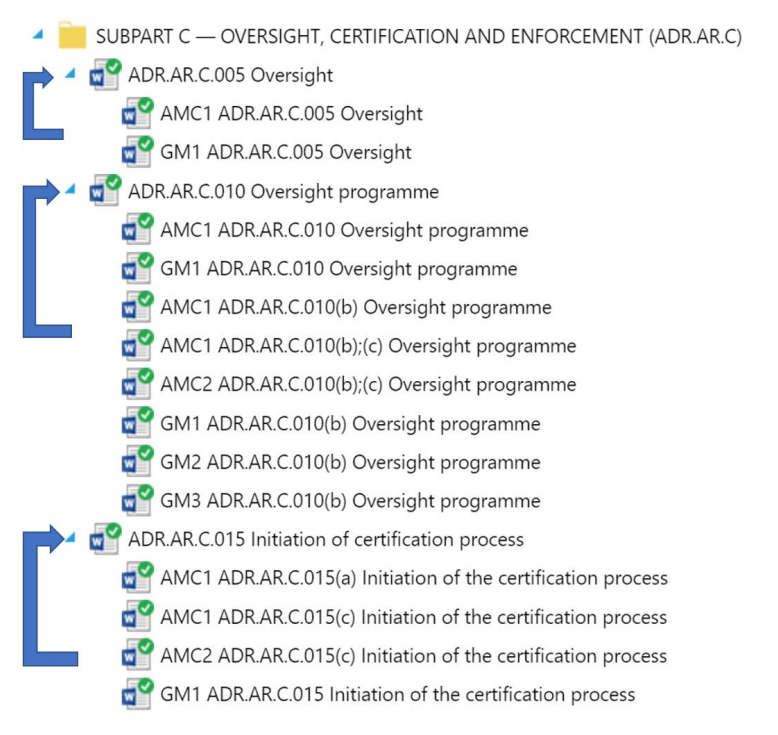
\includegraphics[width=0.75\linewidth]{gfx/parentir.png}
        \caption{Referenzierung des ParentIR Attributs im EASA CCMS}
                                                                                    \cite[31]{easa_xml_doc}
        \label{fig:parent_ir}
    \end{figure}

    

    % \subsection{Vor- \& Nachteile}
    \pagebreak
    \section{Bewertung der Datenquelle}

    Die \acf{EASA} erarbeitet, auf Basis ihrer definierten Aufgaben, \textit{Annehmbare Nachweisverfahren} und \textit{Guidance Material}.
    Um die allgemeine Integration ihrer Daten fortlaufend zu stärken, ist die \ac{EASA} bemüht,  Nutzer:innen nützliche Informationen in zugänglichen und maschinenlesbaren Formaten bereitzustellen. 
    Um die Leserlichkeit und die Verknüpfung von Daten zu vereinfachen, werden die Kombination von Publikationen der \ac{EASA} und den entsprechenden Durchführungsbestimmungen der \ac{EU} in der Form von \acf{EAR} veröffentlicht.
    Diese sollen Stakeholder:innen einen aktuellen Gesamtüberblick über das entsprechende Themengebiet vermitteln und beinhaltet -- im XML Format -- ausgewählte Metadaten aus dem internen \ac{CCMS} der \ac{EASA}.
    


\subsection{Integration in das erarbeitete Datenmodell}

Anders als der analysierte Datensatz auf Basis der \ac{EU} und \textit{Cellar} beruhen die Informationen, welche dieser Quelle entnommen werden -- mit Ausnahme des Inhaltes -- auf einer Datenquelle.
Das hierzu publizierte -- und durch dieses Kapitel analysierte -- Datenschema (Version 1.0.0), beschreibt hierbei die einzelnen Informationen, welche durch die \ac{EASA} annotiert und publiziert werden.
Im Weiteren soll die Abbildung dieser Informationen auf das erarbeitete Anforderungsmodell übertragen werden.

\subsubsection{Eindeutige Kennung}

Die \ac{EAR} Metadaten stellen durch das analysierte \textit{ERulesId} Attribut bereits eine eindeutige Kennung für alle \textit{Topics} -- darunter auch die relevanten Anforderungen der Durchführungsbestimmung -- bereit.
Dieses erfüllt im Rahmen des Modells bereits die Anforderungen, unabhängig von der Struktur und global einzigartig zu sein. 
Im Weiteren ermöglicht es diese Identifizierungsmethode auch, dass Anforderungen in ein anderes Anforderungsdokument übertragen werden können, ohne dass bestehende Referenzen im Rahmen des Nachweisführungsprozesses verloren gehen.

\subsubsection{Regulative Quelle}

Die Regulative Quelle wird im Rahmen der \ac{EAR} \textit{Topics} anhand des \textit{RegulatorySource} Attributs bestimmt. 
Diese Angabe wird, als einer der weniger, auch in den anderen Formaten der \acp{EAR} angegeben und bestimmt, nach der Analyse (siehe \ref{ch:easa_anal}) den Rechtsakt, welcher diese Anforderung publiziert oder -- im Rahmen von Änderungen -- zuletzt konsolidiert hat. 

\pagebreak
\subsubsection{Inkrafttreten / Anwendungszeitraum}

Auch die Angaben zum Anwendungszeitraum gehen explizit aus den Daten hervor. 
So definieren die Attribute \textit{Applicability-} und \textit{EntryIntoForceDate} bereits das Ende der Übergangsperiode und das rechtliche Inkrafttreten der Anforderung ab, auf Basis welcher ein Anwendungszeitraum (gemäß \ref{model_anforderungen}) angenommen werden kann.

\subsubsection{Lifecycle}

Die \ac{EAR} bilden immer nur den aktuellen Zustand aller Anforderungen, und dessen Zusatzmaterialien, ab.
Eine Versionierung der einzelnen \textit{Topics} ist hiernach intern zwar vorhanden, jedoch nicht offen zugänglich\footnote{Die \ac{EASA} hat im Interview vorbehalten weitere Daten des \ac{CCMS} zu veröffentlichen, sowie ein Interesse der Nutzer:innen besteht (siehe \ref{ch:ausblick}) \cite{easa_xml_export}.}.
Dies ermöglicht keine direkte Abbildung eines Lifecycles oder bspw. der Referenzierung von inaktiven\footnote{Nicht mehr in Kraft} Anforderungen, da diese in neuen Publikationen des \ac{EAR}-Formates nicht mehr enthalten sind.
Die Abbildung 
Angaben der Metadaten wie die \textit{Regulative Quelle} oder @AmendedBy (siehe \ref{ch:easa_anal}) erlauben es jedoch, nachzuvollziehen, wann eine Anforderung publiziert und geändert wurde.

\subsection{Verfügbarkeit und rechtliche Verbindlichkeit}

    Die große Schwachstelle dieser Datenquelle besteht in deren Verfügbarkeit und rechtliche Verbindlichkeit.
    Die \ac{EASA} kuriert folglich nur ausgewählte Durchführungsbestimmungen und publiziert nach der Entwicklung oder Anpassung entsprechender \textit{Annehmbaren Nachweisverfahren} und \textit{Guidance Materials} dessen neue Version für alle Nutzer:innen.
    Diese Entwicklung ist rechtlich nicht an einen zeitlichen Rahmen gebunden, weshalb die Bereitstellung der Daten zu dem Inkrafttreten der Bestimmungen nicht garantiert ist\footnote{Zum aktuellen Zeitpunkt (02/2024) wurden die Änderungen der \vo{DVO}{EU}{2023/1771} bzgl. der \vo{DVO}{EU}{2017/373} aus 09/2023 noch nicht auf die entsprechende \ac{EAR} (Easy Access Rule for \atmans) übertragen.}.
    Auch wenn es offen bleibt, inwiefern die Behörden gegen veraltete Angaben, basierend auf dem eigenen Datensatz vorgehenden würden, so ist es rechtlich klar abgesteckt, dass der rechtliche Sollzustand durch die geltenden Durchführungsbestimmungen definiert wird.
    Die \ac{EAR}\footnote{formatunabhängig} bilden dabei lediglich eine Präsentationsschicht dieser Daten, welche Nutzer:innen einen einfacheren Zugang zu diesen ermöglichen soll. 
    Die rechtliche Verbindlichkeit diese Angaben sind durch die \ac{EASA} ganz klar eingeschränkt:

\begin{quote}
    ,,Easy Access Rules (in any of the available formats) are not an official publication. Only European Union documents published in the Official Journal of the European Union are deemed authentic.``\footnote{Zur Regulierung der Authentizität des \ac{OJ} siehe \vo{VO}{EU}{216/2013} des Rates} \cite{easa_xml_export}
\end{quote}
    
     